\documentclass[twoside]{book}

% Packages required by doxygen
\usepackage{fixltx2e}
\usepackage{calc}
\usepackage{doxygen}
\usepackage[export]{adjustbox} % also loads graphicx
\usepackage{graphicx}
\usepackage[utf8]{inputenc}
\usepackage{makeidx}
\usepackage{multicol}
\usepackage{multirow}
\PassOptionsToPackage{warn}{textcomp}
\usepackage{textcomp}
\usepackage[nointegrals]{wasysym}
\usepackage[table]{xcolor}

% Font selection
\usepackage[T1]{fontenc}
\usepackage[scaled=.90]{helvet}
\usepackage{courier}
\usepackage{amssymb}
\usepackage{sectsty}
\renewcommand{\familydefault}{\sfdefault}
\allsectionsfont{%
  \fontseries{bc}\selectfont%
  \color{darkgray}%
}
\renewcommand{\DoxyLabelFont}{%
  \fontseries{bc}\selectfont%
  \color{darkgray}%
}
\newcommand{\+}{\discretionary{\mbox{\scriptsize$\hookleftarrow$}}{}{}}

% Page & text layout
\usepackage{geometry}
\geometry{%
  a4paper,%
  top=2.5cm,%
  bottom=2.5cm,%
  left=2.5cm,%
  right=2.5cm%
}
\tolerance=750
\hfuzz=15pt
\hbadness=750
\setlength{\emergencystretch}{15pt}
\setlength{\parindent}{0cm}
\setlength{\parskip}{0.2cm}
\makeatletter
\renewcommand{\paragraph}{%
  \@startsection{paragraph}{4}{0ex}{-1.0ex}{1.0ex}{%
    \normalfont\normalsize\bfseries\SS@parafont%
  }%
}
\renewcommand{\subparagraph}{%
  \@startsection{subparagraph}{5}{0ex}{-1.0ex}{1.0ex}{%
    \normalfont\normalsize\bfseries\SS@subparafont%
  }%
}
\makeatother

% Headers & footers
\usepackage{fancyhdr}
\pagestyle{fancyplain}
\fancyhead[LE]{\fancyplain{}{\bfseries\thepage}}
\fancyhead[CE]{\fancyplain{}{}}
\fancyhead[RE]{\fancyplain{}{\bfseries\leftmark}}
\fancyhead[LO]{\fancyplain{}{\bfseries\rightmark}}
\fancyhead[CO]{\fancyplain{}{}}
\fancyhead[RO]{\fancyplain{}{\bfseries\thepage}}
\fancyfoot[LE]{\fancyplain{}{}}
\fancyfoot[CE]{\fancyplain{}{}}
\fancyfoot[RE]{\fancyplain{}{\bfseries\scriptsize Generated on Sun Dec 20 2015 09\+:08\+:38 for L\+Pad by Doxygen }}
\fancyfoot[LO]{\fancyplain{}{\bfseries\scriptsize Generated on Sun Dec 20 2015 09\+:08\+:38 for L\+Pad by Doxygen }}
\fancyfoot[CO]{\fancyplain{}{}}
\fancyfoot[RO]{\fancyplain{}{}}
\renewcommand{\footrulewidth}{0.4pt}
\renewcommand{\chaptermark}[1]{%
  \markboth{#1}{}%
}
\renewcommand{\sectionmark}[1]{%
  \markright{\thesection\ #1}%
}

% Indices & bibliography
\usepackage{natbib}
\usepackage[titles]{tocloft}
\setcounter{tocdepth}{3}
\setcounter{secnumdepth}{5}
\makeindex

% Hyperlinks (required, but should be loaded last)
\usepackage{ifpdf}
\ifpdf
  \usepackage[pdftex,pagebackref=true]{hyperref}
\else
  \usepackage[ps2pdf,pagebackref=true]{hyperref}
\fi
\hypersetup{%
  colorlinks=true,%
  linkcolor=blue,%
  citecolor=blue,%
  unicode%
}

% Custom commands
\newcommand{\clearemptydoublepage}{%
  \newpage{\pagestyle{empty}\cleardoublepage}%
}


%===== C O N T E N T S =====

\begin{document}

% Titlepage & ToC
\hypersetup{pageanchor=false,
             bookmarks=true,
             bookmarksnumbered=true,
             pdfencoding=unicode
            }
\pagenumbering{roman}
\begin{titlepage}
\vspace*{7cm}
\begin{center}%
{\Large L\+Pad \\[1ex]\large 0.\+1v }\\
\vspace*{1cm}
{\large Generated by Doxygen 1.8.10}\\
\vspace*{0.5cm}
{\small Sun Dec 20 2015 09:08:38}\\
\end{center}
\end{titlepage}
\clearemptydoublepage
\tableofcontents
\clearemptydoublepage
\pagenumbering{arabic}
\hypersetup{pageanchor=true}

%--- Begin generated contents ---
\chapter{Hierarchical Index}
\section{Class Hierarchy}
This inheritance list is sorted roughly, but not completely, alphabetically\+:\begin{DoxyCompactList}
\item Q\+Dialog\begin{DoxyCompactList}
\item \contentsline{section}{about}{\pageref{classabout}}{}
\item \contentsline{section}{wordfind}{\pageref{classwordfind}}{}
\end{DoxyCompactList}
\item Q\+Main\+Window\begin{DoxyCompactList}
\item \contentsline{section}{L\+Pad}{\pageref{class_l_pad}}{}
\end{DoxyCompactList}
\end{DoxyCompactList}

\chapter{Class Index}
\section{Class List}
Here are the classes, structs, unions and interfaces with brief descriptions\+:\begin{DoxyCompactList}
\item\contentsline{section}{\hyperlink{classabout}{about} }{\pageref{classabout}}{}
\item\contentsline{section}{\hyperlink{class_l_pad}{L\+Pad} }{\pageref{class_l_pad}}{}
\item\contentsline{section}{\hyperlink{classwordfind}{wordfind} }{\pageref{classwordfind}}{}
\end{DoxyCompactList}

\chapter{Class Documentation}
\hypertarget{classabout}{}\section{about Class Reference}
\label{classabout}\index{about@{about}}
Inheritance diagram for about\+:\begin{figure}[H]
\begin{center}
\leavevmode
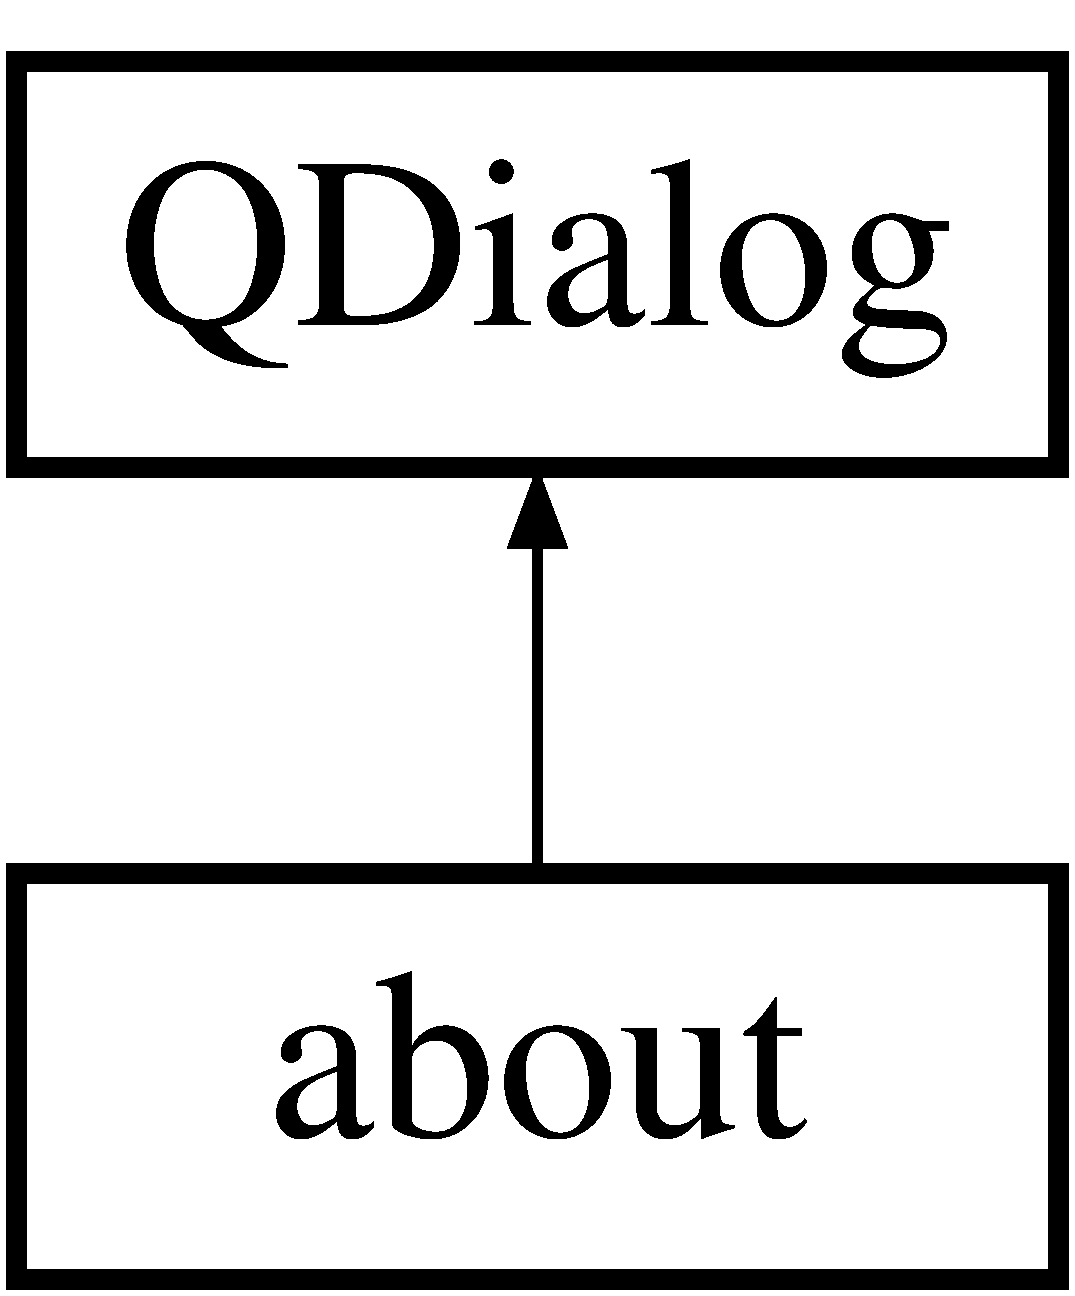
\includegraphics[height=2.000000cm]{classabout}
\end{center}
\end{figure}
\subsection*{Public Member Functions}
\begin{DoxyCompactItemize}
\item 
\hypertarget{classabout_ab16a8ec628d97aee17f0332e09964f52}{}{\bfseries about} (Q\+Widget $\ast$parent=0)\label{classabout_ab16a8ec628d97aee17f0332e09964f52}

\end{DoxyCompactItemize}


The documentation for this class was generated from the following files\+:\begin{DoxyCompactItemize}
\item 
C\+:/\+Users/\+Lahiru/\+Documents/\+Qt projects/\+L\+Pad/about.\+h\item 
C\+:/\+Users/\+Lahiru/\+Documents/\+Qt projects/\+L\+Pad/about.\+cpp\end{DoxyCompactItemize}

\hypertarget{class_l_pad}{}\section{L\+Pad Class Reference}
\label{class_l_pad}\index{L\+Pad@{L\+Pad}}
Inheritance diagram for L\+Pad\+:\begin{figure}[H]
\begin{center}
\leavevmode
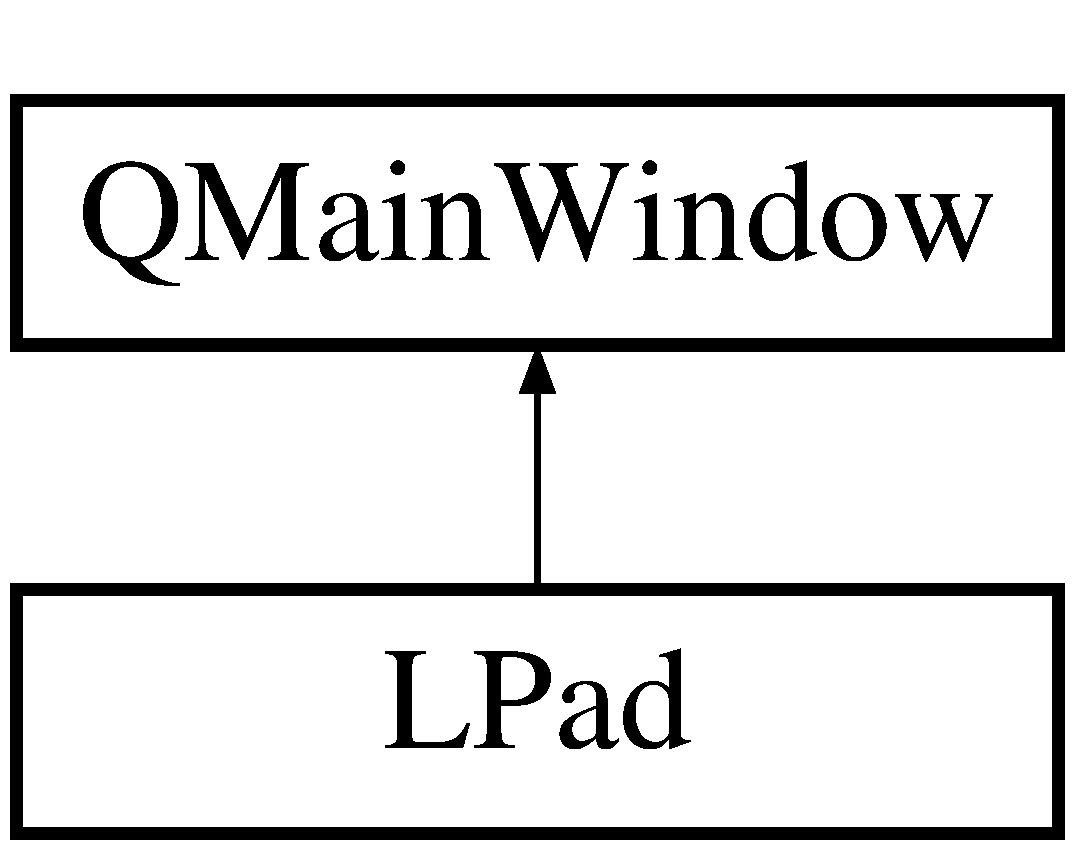
\includegraphics[height=2.000000cm]{class_l_pad}
\end{center}
\end{figure}
\subsection*{Public Slots}
\begin{DoxyCompactItemize}
\item 
\hypertarget{class_l_pad_ae424b390470d27f9942e526e9cabcfa8}{}void \hyperlink{class_l_pad_ae424b390470d27f9942e526e9cabcfa8}{print\+File} ()\label{class_l_pad_ae424b390470d27f9942e526e9cabcfa8}

\begin{DoxyCompactList}\small\item\em \hyperlink{class_l_pad_ae424b390470d27f9942e526e9cabcfa8}{L\+Pad\+::print\+File}. \end{DoxyCompactList}\item 
\hypertarget{class_l_pad_aa2194ad36d99f7f2174cb72ca267fe62}{}void \hyperlink{class_l_pad_aa2194ad36d99f7f2174cb72ca267fe62}{openfile} ()\label{class_l_pad_aa2194ad36d99f7f2174cb72ca267fe62}

\begin{DoxyCompactList}\small\item\em \hyperlink{class_l_pad_aa2194ad36d99f7f2174cb72ca267fe62}{L\+Pad\+::openfile}. \end{DoxyCompactList}\item 
\hypertarget{class_l_pad_a97d2edc85951c083b45afe121d1dce71}{}void \hyperlink{class_l_pad_a97d2edc85951c083b45afe121d1dce71}{newfile} ()\label{class_l_pad_a97d2edc85951c083b45afe121d1dce71}

\begin{DoxyCompactList}\small\item\em \hyperlink{class_l_pad_a97d2edc85951c083b45afe121d1dce71}{L\+Pad\+::newfile}. \end{DoxyCompactList}\item 
\hypertarget{class_l_pad_a9bed2655dcdbfe683ce7f50917adfc55}{}void \hyperlink{class_l_pad_a9bed2655dcdbfe683ce7f50917adfc55}{get\+Text\+File} ()\label{class_l_pad_a9bed2655dcdbfe683ce7f50917adfc55}

\begin{DoxyCompactList}\small\item\em \hyperlink{class_l_pad_a9bed2655dcdbfe683ce7f50917adfc55}{L\+Pad\+::get\+Text\+File}. \end{DoxyCompactList}\item 
bool \hyperlink{class_l_pad_a86ee706e6d0a422366fe8752e7ae7213}{saveasfile} ()
\begin{DoxyCompactList}\small\item\em \hyperlink{class_l_pad_a86ee706e6d0a422366fe8752e7ae7213}{L\+Pad\+::saveasfile}. \end{DoxyCompactList}\item 
bool \hyperlink{class_l_pad_af616501190be280a535b667e450ed914}{savefile} ()
\begin{DoxyCompactList}\small\item\em \hyperlink{class_l_pad_af616501190be280a535b667e450ed914}{L\+Pad\+::savefile}. \end{DoxyCompactList}\end{DoxyCompactItemize}
\subsection*{Public Member Functions}
\begin{DoxyCompactItemize}
\item 
\hyperlink{class_l_pad_ae4d17da9ca09a5c0dbcebc20f1d981c9}{L\+Pad} (Q\+Widget $\ast$parent=0)
\begin{DoxyCompactList}\small\item\em \hyperlink{class_l_pad_ae4d17da9ca09a5c0dbcebc20f1d981c9}{L\+Pad\+::\+L\+Pad}. \end{DoxyCompactList}\item 
\hypertarget{class_l_pad_a3379f0db7845c9cebbab6b365d3b855f}{}\hyperlink{class_l_pad_a3379f0db7845c9cebbab6b365d3b855f}{$\sim$\+L\+Pad} ()\label{class_l_pad_a3379f0db7845c9cebbab6b365d3b855f}

\begin{DoxyCompactList}\small\item\em \hyperlink{class_l_pad_a3379f0db7845c9cebbab6b365d3b855f}{L\+Pad\+::$\sim$\+L\+Pad}. \end{DoxyCompactList}\item 
\hypertarget{class_l_pad_a702aadf33cff4f2ab7c6e9afe9ecd2cd}{}void {\bfseries find\+Word} (Q\+String word)\label{class_l_pad_a702aadf33cff4f2ab7c6e9afe9ecd2cd}

\end{DoxyCompactItemize}
\subsection*{Public Attributes}
\begin{DoxyCompactItemize}
\item 
\hypertarget{class_l_pad_a0c9ea7dd98b870c806ec09957b23c110}{}Q\+String {\bfseries m\+Filename}\label{class_l_pad_a0c9ea7dd98b870c806ec09957b23c110}

\end{DoxyCompactItemize}
\subsection*{Protected Member Functions}
\begin{DoxyCompactItemize}
\item 
void \hyperlink{class_l_pad_a3c1505476d5c4a12a5b9015c37c3afca}{close\+Event} (Q\+Close\+Event $\ast$event)
\begin{DoxyCompactList}\small\item\em \hyperlink{class_l_pad_a3c1505476d5c4a12a5b9015c37c3afca}{L\+Pad\+::close\+Event}. \end{DoxyCompactList}\end{DoxyCompactItemize}


\subsection{Constructor \& Destructor Documentation}
\hypertarget{class_l_pad_ae4d17da9ca09a5c0dbcebc20f1d981c9}{}\index{L\+Pad@{L\+Pad}!L\+Pad@{L\+Pad}}
\index{L\+Pad@{L\+Pad}!L\+Pad@{L\+Pad}}
\subsubsection[{L\+Pad(\+Q\+Widget $\ast$parent=0)}]{\setlength{\rightskip}{0pt plus 5cm}L\+Pad\+::\+L\+Pad (
\begin{DoxyParamCaption}
\item[{Q\+Widget $\ast$}]{parent = {\ttfamily 0}}
\end{DoxyParamCaption}
)\hspace{0.3cm}{\ttfamily [explicit]}}\label{class_l_pad_ae4d17da9ca09a5c0dbcebc20f1d981c9}


\hyperlink{class_l_pad_ae4d17da9ca09a5c0dbcebc20f1d981c9}{L\+Pad\+::\+L\+Pad}. 


\begin{DoxyParams}{Parameters}
{\em parent} & \\
\hline
\end{DoxyParams}


\subsection{Member Function Documentation}
\hypertarget{class_l_pad_a3c1505476d5c4a12a5b9015c37c3afca}{}\index{L\+Pad@{L\+Pad}!close\+Event@{close\+Event}}
\index{close\+Event@{close\+Event}!L\+Pad@{L\+Pad}}
\subsubsection[{close\+Event(\+Q\+Close\+Event $\ast$event)}]{\setlength{\rightskip}{0pt plus 5cm}void L\+Pad\+::close\+Event (
\begin{DoxyParamCaption}
\item[{Q\+Close\+Event $\ast$}]{event}
\end{DoxyParamCaption}
)\hspace{0.3cm}{\ttfamily [protected]}}\label{class_l_pad_a3c1505476d5c4a12a5b9015c37c3afca}


\hyperlink{class_l_pad_a3c1505476d5c4a12a5b9015c37c3afca}{L\+Pad\+::close\+Event}. 


\begin{DoxyParams}{Parameters}
{\em event} & \\
\hline
\end{DoxyParams}
\hypertarget{class_l_pad_a86ee706e6d0a422366fe8752e7ae7213}{}\index{L\+Pad@{L\+Pad}!saveasfile@{saveasfile}}
\index{saveasfile@{saveasfile}!L\+Pad@{L\+Pad}}
\subsubsection[{saveasfile}]{\setlength{\rightskip}{0pt plus 5cm}bool L\+Pad\+::saveasfile (
\begin{DoxyParamCaption}
{}
\end{DoxyParamCaption}
)\hspace{0.3cm}{\ttfamily [slot]}}\label{class_l_pad_a86ee706e6d0a422366fe8752e7ae7213}


\hyperlink{class_l_pad_a86ee706e6d0a422366fe8752e7ae7213}{L\+Pad\+::saveasfile}. 

\begin{DoxyReturn}{Returns}

\end{DoxyReturn}
\hypertarget{class_l_pad_af616501190be280a535b667e450ed914}{}\index{L\+Pad@{L\+Pad}!savefile@{savefile}}
\index{savefile@{savefile}!L\+Pad@{L\+Pad}}
\subsubsection[{savefile}]{\setlength{\rightskip}{0pt plus 5cm}bool L\+Pad\+::savefile (
\begin{DoxyParamCaption}
{}
\end{DoxyParamCaption}
)\hspace{0.3cm}{\ttfamily [slot]}}\label{class_l_pad_af616501190be280a535b667e450ed914}


\hyperlink{class_l_pad_af616501190be280a535b667e450ed914}{L\+Pad\+::savefile}. 

\begin{DoxyReturn}{Returns}

\end{DoxyReturn}


The documentation for this class was generated from the following files\+:\begin{DoxyCompactItemize}
\item 
C\+:/\+Users/\+Lahiru/\+Documents/\+Qt projects/\+L\+Pad/lpad.\+h\item 
C\+:/\+Users/\+Lahiru/\+Documents/\+Qt projects/\+L\+Pad/lpad.\+cpp\end{DoxyCompactItemize}

\hypertarget{classwordfind}{}\section{wordfind Class Reference}
\label{classwordfind}\index{wordfind@{wordfind}}
Inheritance diagram for wordfind\+:\begin{figure}[H]
\begin{center}
\leavevmode
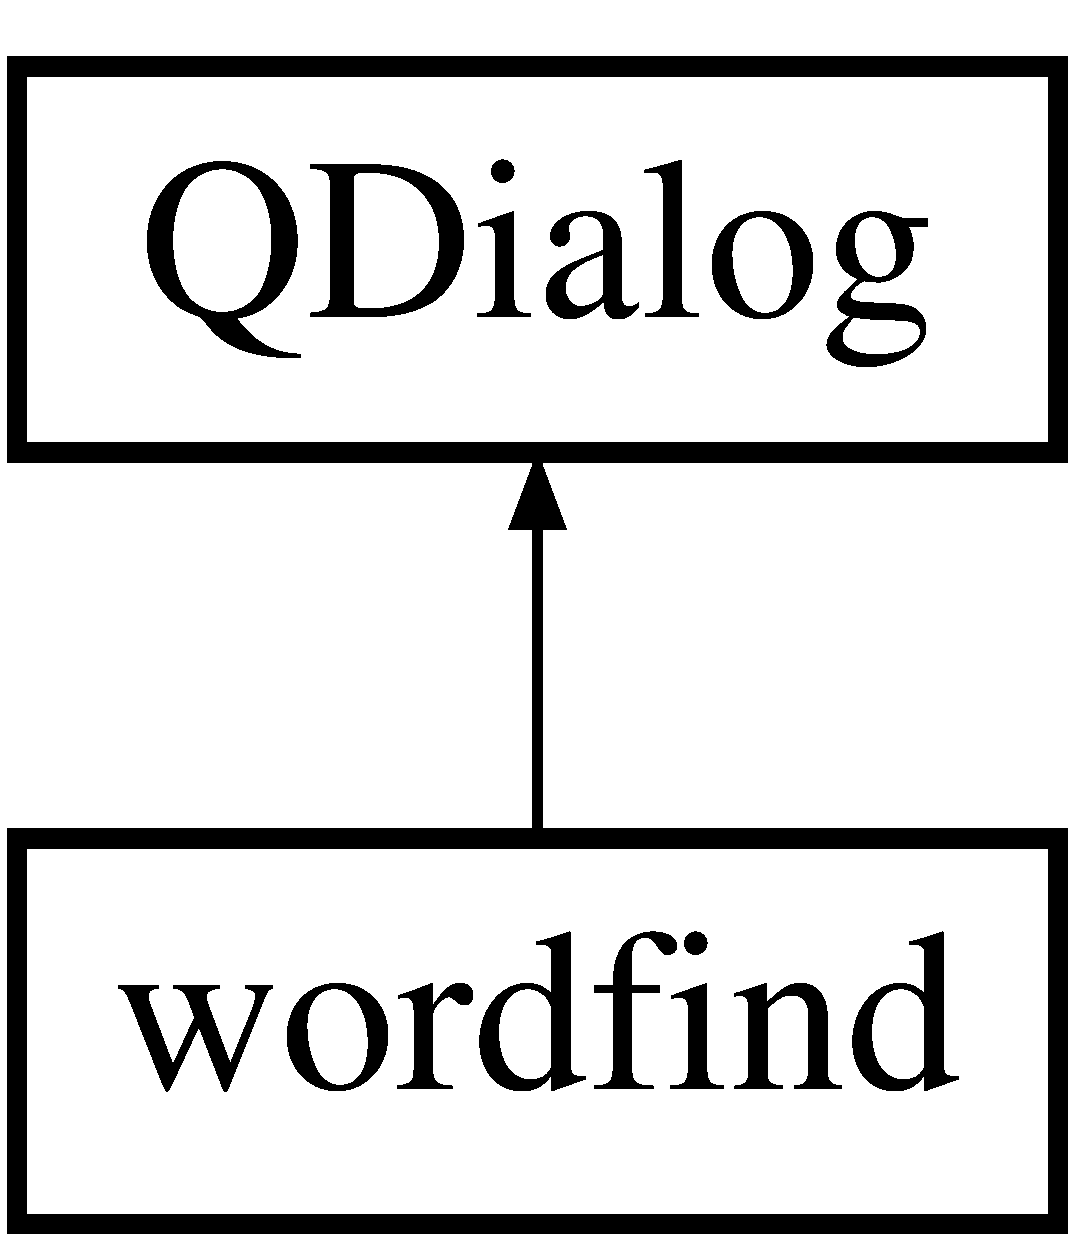
\includegraphics[height=2.000000cm]{classwordfind}
\end{center}
\end{figure}
\subsection*{Public Member Functions}
\begin{DoxyCompactItemize}
\item 
\hypertarget{classwordfind_a9f53971bfab9ec3ea7480c5eec5c79fc}{}{\bfseries wordfind} (Q\+Widget $\ast$parent=0)\label{classwordfind_a9f53971bfab9ec3ea7480c5eec5c79fc}

\end{DoxyCompactItemize}


The documentation for this class was generated from the following files\+:\begin{DoxyCompactItemize}
\item 
C\+:/\+Users/\+Lahiru/\+Documents/\+Qt projects/\+L\+Pad/wordfind.\+h\item 
C\+:/\+Users/\+Lahiru/\+Documents/\+Qt projects/\+L\+Pad/wordfind.\+cpp\end{DoxyCompactItemize}

%--- End generated contents ---

% Index
\backmatter
\newpage
\phantomsection
\clearemptydoublepage
\addcontentsline{toc}{chapter}{Index}
\printindex

\end{document}
